\documentclass{beamer}
%\usetheme{Singapore}
\usetheme{Darmstadt}
\useoutertheme{smoothtree}
\setbeamertemplate{footline}[page number]{}
\beamertemplateballitem
\usepackage{graphicx}
\usepackage{subfigure}
\usepackage{bm}
\usepackage{array,amsmath,latexsym,epsfig,float,afterpage,alltt,amssymb,theorem,enumerate,pstricks,bm,hhline,url,xr,float,multicol,multirow,ragged2e,colortbl,xspace, natbib}
\graphicspath{{figs/}}

\newcommand{\Blue}{\color{blue}}
\newcommand{\Red}{\color{red}}
\newcommand{\Green}{\color{green}}
\def\1{{\bf 1}}\def\rkhs{{\cal H}}

% Example definitions.
% --------------------

\def\cL{{\cal L}}
\def\cU{{\cal U}}
\def\cF{{\cal F}}
\def\cM{{\cal M}}
\def\cC{{\cal C}}
\def\cD{{\cal D}}
\def\cA{{\cal A}}


\def\bR{{\boldsymbol R}}
\def\bS{{\boldsymbol S}}
\def\bJ{{\boldsymbol J}}
\def\ba{{\boldsymbol a}}
\def\bb{{\boldsymbol b}}
\def\bw{{\boldsymbol w}}
\def\bu{{\boldsymbol u}}
\def\balpha{{\boldsymbol \alpha}}
\def\bbeta{{\boldsymbol \beta}}
\def\bd{{\boldsymbol d}}
\def\bb{{\boldsymbol b}}
\def\be{{\boldsymbol e}}
\def\bp{{\boldsymbol p}}
\def\bzero{{\boldsymbol 0}}
\def\bx{{\boldsymbol x}}
\def\by{{\boldsymbol y}}
\def\bv{{\boldsymbol v}}
\def\bq{{\boldsymbol q}}
\def\bxi{{\boldsymbol \xi}}
\def\liblinear{{{\sf LIBLINEAR}\xspace}}
\def\vw{{\sf VW}\xspace}
\def\pegasos{{\sf PEGASOS}\xspace}
\def\libsvm{{\sf LIBSVM}\xspace}

\def\bX{{\mathbf X}}
\def\x{{\mathbf x}}
\def\L{{\cal L}}

\AtBeginSubsection[]
{
    \begin{frame}<beamer>
        \frametitle{Outline}
        \tableofcontents[current,currentsubsection]
    \end{frame}
}


\begin{document}
\section{ }
\title[Nystr\"om Decomposition]{Solving Non-Linear SVM in Linear Time? -- A Nystr\"om Approximated SVM with Applications to Image Classification}
\author[Ming-Hen Tsai]{
{\scriptsize
Ming-Hen Tsai, Academia Sinica, Taiwan (now at Google Inc.)\\
Joint work with \\
Yi-Ren Yeh, Intel-NTU Connected Context Computing Center \\
Yuh-Jye Lee, Dept. CSIE, National Taiwan University Science \& Technology\\
Yu-Chiang Frank Wang, Research Center for IT Innovation, Academia Sinica\\
}
}
\date{May 21, 2013}


%%-----------------------------------------------
%\begin{frame}
%\end{frame}


%-----------------------------------------------
\begin{frame}
\titlepage
\end{frame}

%%-----------------------------------------------
\begin{frame}{Outline}
\tableofcontents[pausesections]
\end{frame}

%-----------------------------------------------
\subsection{Introduction}

\begin{frame}
  \frametitle{Visual Classification: Faces, Objects, and Beyond}
  \begin{figure}
  % Requires \usepackage{graphicx}
  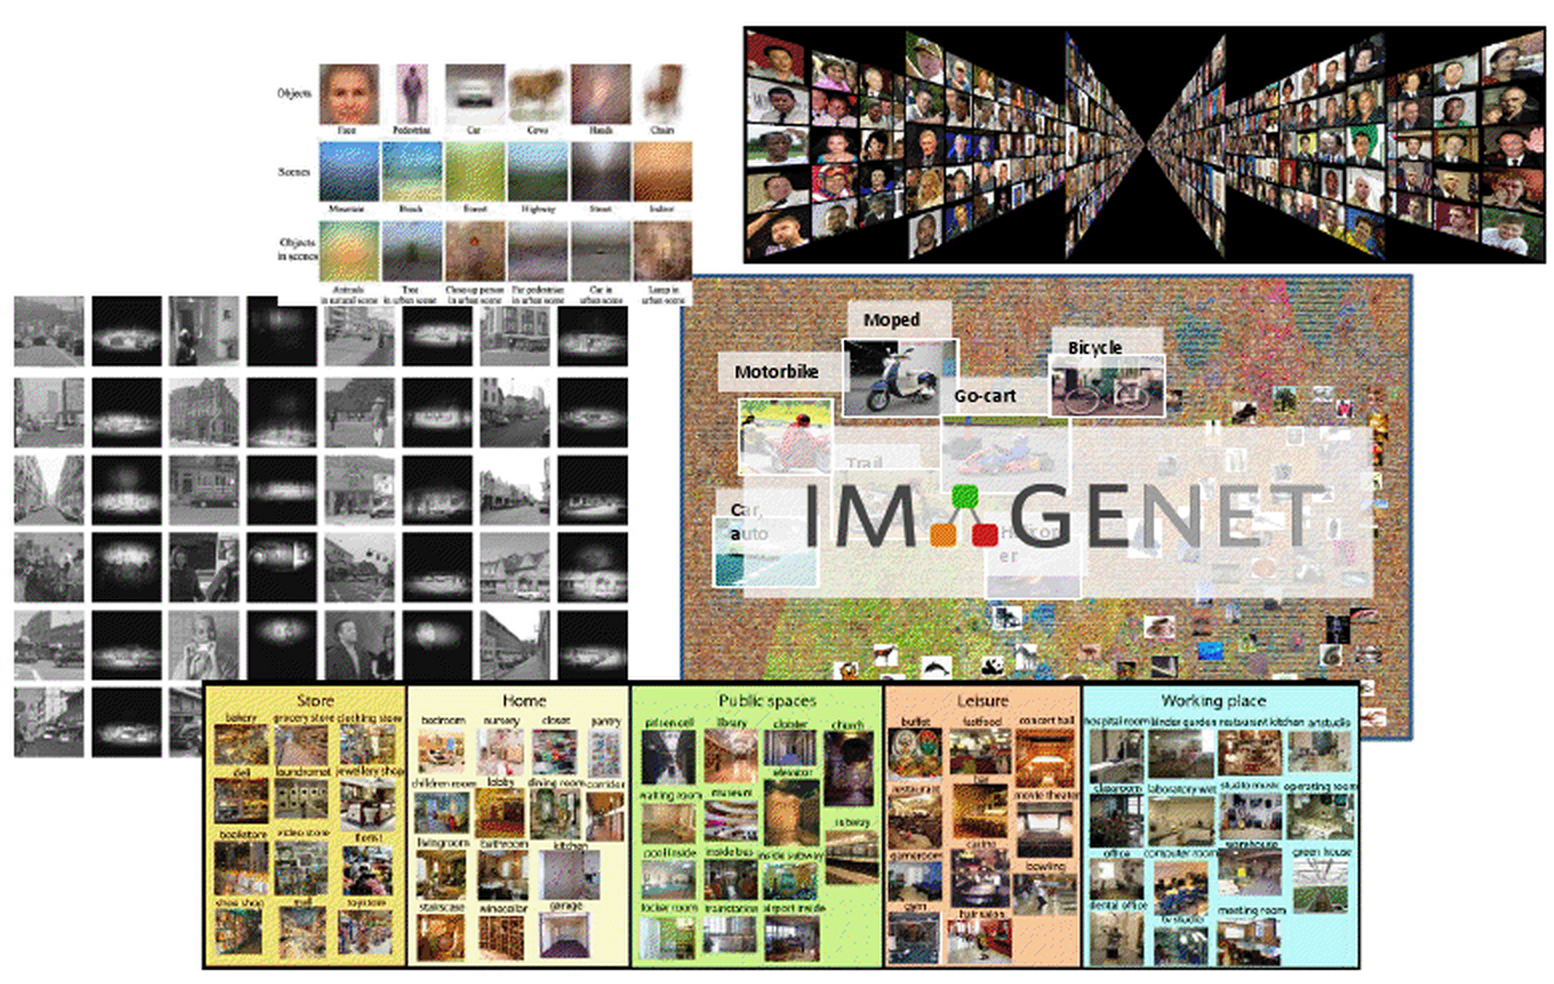
\includegraphics[width=4in]{tasks_illus.png}\\
  \end{figure}
\end{frame}

\begin{frame}
  \frametitle{Example: Some Image Classification Data Sets}
  \begin{figure}
  % Requires \usepackage{graphicx}
  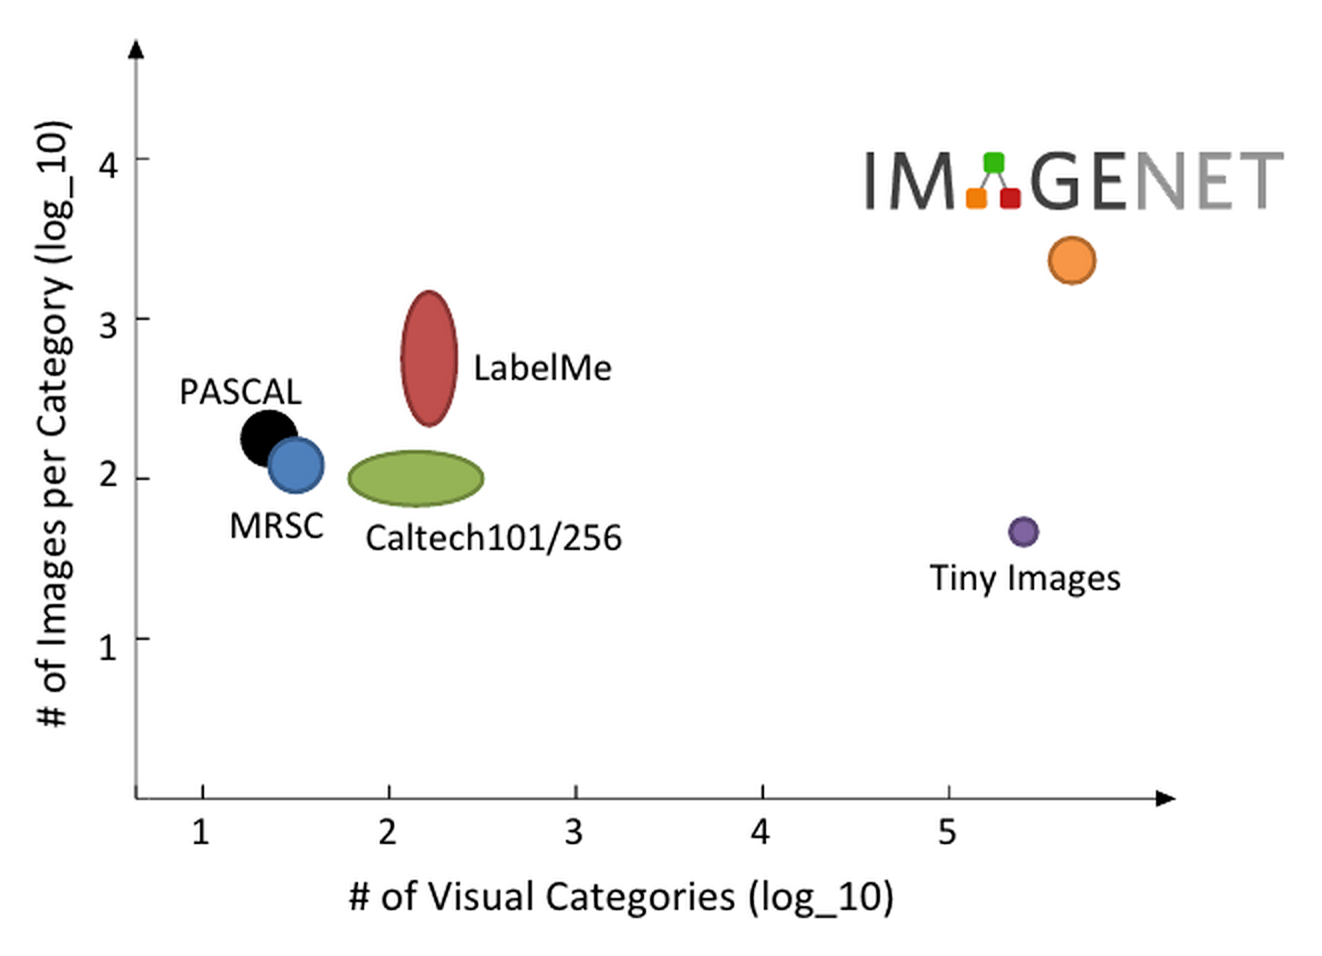
\includegraphics[width=4in]{tasks_summary.png}\\
  \end{figure}
\end{frame}

\begin{frame}
  \frametitle{We Have Known...}
  \begin{itemize}
    \item Non-linear SVM: powerful but slow 
    \item Linear SVM: simple but fast  
    \item [] Paper: "Training Linear SVMs in Linear Time" by Joachims
    \item [] Software: \liblinear, \vw, etc.
 \end{itemize}
\end{frame}

\begin{frame}
  \frametitle{We Had Always Wondered...}
  \begin{itemize}
    \item But we want something {\bf powerful} and {\bf fast}: train faster than non-linear SVM and generate a more accurate model than linear SVM.
    \pause
    \item [] What should we do? 
    \pause
    \item Can we save some computations (for speed) and still get non-linearity (for more power)?
    \pause
    \item [] Yes. Do approximation!
  \end{itemize}
\end{frame}


\subsection{Nystr\"om Method for Kernel Approximation}
\begin{frame}
  \frametitle{Definitions and a Brief Review (1/2)}
  \begin{itemize}
    \item Input Data: $\{(\by, X)\} = \{(y_i, \bx_i)\}_{i=1}^\ell$. $y_i$: label, $\bx_i$: feature vector.
    \item (Non-zero) dimension of $\bx_i$: $n$
    \item Non-linear mapping $\phi(\bx)$ (e.g. bi-gram features)
    \item Kernel function: $K(\bu, \bv) = \phi(\bu)^T \phi(\bv)$, usually computed in linear time.
    \item For ease of representaion, for $U = [\bu_1, \dots, \bu_\ell]$ and $V = [\bv_1, \dots, \bv_{\tilde{\ell}}]$, we define $Q = K(U, V)$, where $Q_{ij} = K(\bu_i, \bv_j)$
    \pause
    \item Lower bound for data storage and training: $\Omega(\ell n)$.
  \end{itemize}
\end{frame}

\begin{frame}
  \frametitle{Definitions and a Brief Review (2/2)}
  \begin{itemize}
    \item Primal:
    \begin{equation}
      \min_{\bw, b}
      \frac{1}{2} \bw^T\bw + C\sum_{i=1}^\ell \max(1-y_i\bw^T\phi(\bx_i), 0) \nonumber
    \end{equation} 
    \item Dual: 
    \begin{align}
    \min_{\balpha} \  &  \frac{1}{2} \balpha^T Q  \balpha - \be^T \balpha \nonumber \\
    \mbox{s.t.} \  & 0 \le \alpha_i \le C \quad \forall i \mbox{.} \nonumber
    \end{align}
    \item Primal-Dual Correspondence: $\bw = \sum_{i=1}^\ell y_i \alpha_i \phi(\bx_i)$ 
  \end{itemize}
\end{frame}


\begin{frame}
  \frametitle{Kernel in Non-linear SVM}
  \begin{itemize}
    \item Dual form:
    \begin{align}
    \label{eq:svmdual} \nonumber
    \min_{\balpha} \  &  \frac{1}{2} \balpha^T Q  \balpha - \be^T \balpha \nonumber \\
    \mbox{s.t.} \  & 0 \le \alpha_i \le C \quad \forall i \mbox{.} \nonumber
    \end{align}
    \item Kernel matrix $Q$ with $Q_{ij} = K(\bx_i, \bx_j)$.
    \pause
    \item [] Computational time: $O(\ell^2)$ times kernel products $\sim O(\ell^2 n) \sim \ell$ times data size.
    \item [] Space: $O(\ell^2)$.
    \pause
    \item $1M$ images, $1k$ dimensional features: $1M$ times more computational time, and $1M/1k = 1k$ times more space than the linear counterpart.
    % I dont have that resources!!!
  \end{itemize}
\end{frame}

\begin{frame}
  \frametitle{Nystr\"om Method}
  \begin{itemize}
    \item Sample $\tilde{\ell}$ feature vectors from $X$ to a set $B = \{\bb_i\}_{i = 1}^{\tilde{\ell}}$.
    \item The apprxoimated kernel: $Q \sim \tilde{Q} = P^TW^{-1}P$,
    where $P_{ij} = K(\bx_i \bb_j)$ and $W_{ij} = K(\bb_i, \bb_j)$.
%    \item [] so $C$ is $\ell$ by $k$, $W$ is $k$ by $k$. Usually $n \sim k \ll \ell$. 
\begin{figure}
  % Requires \usepackage{graphicx}
  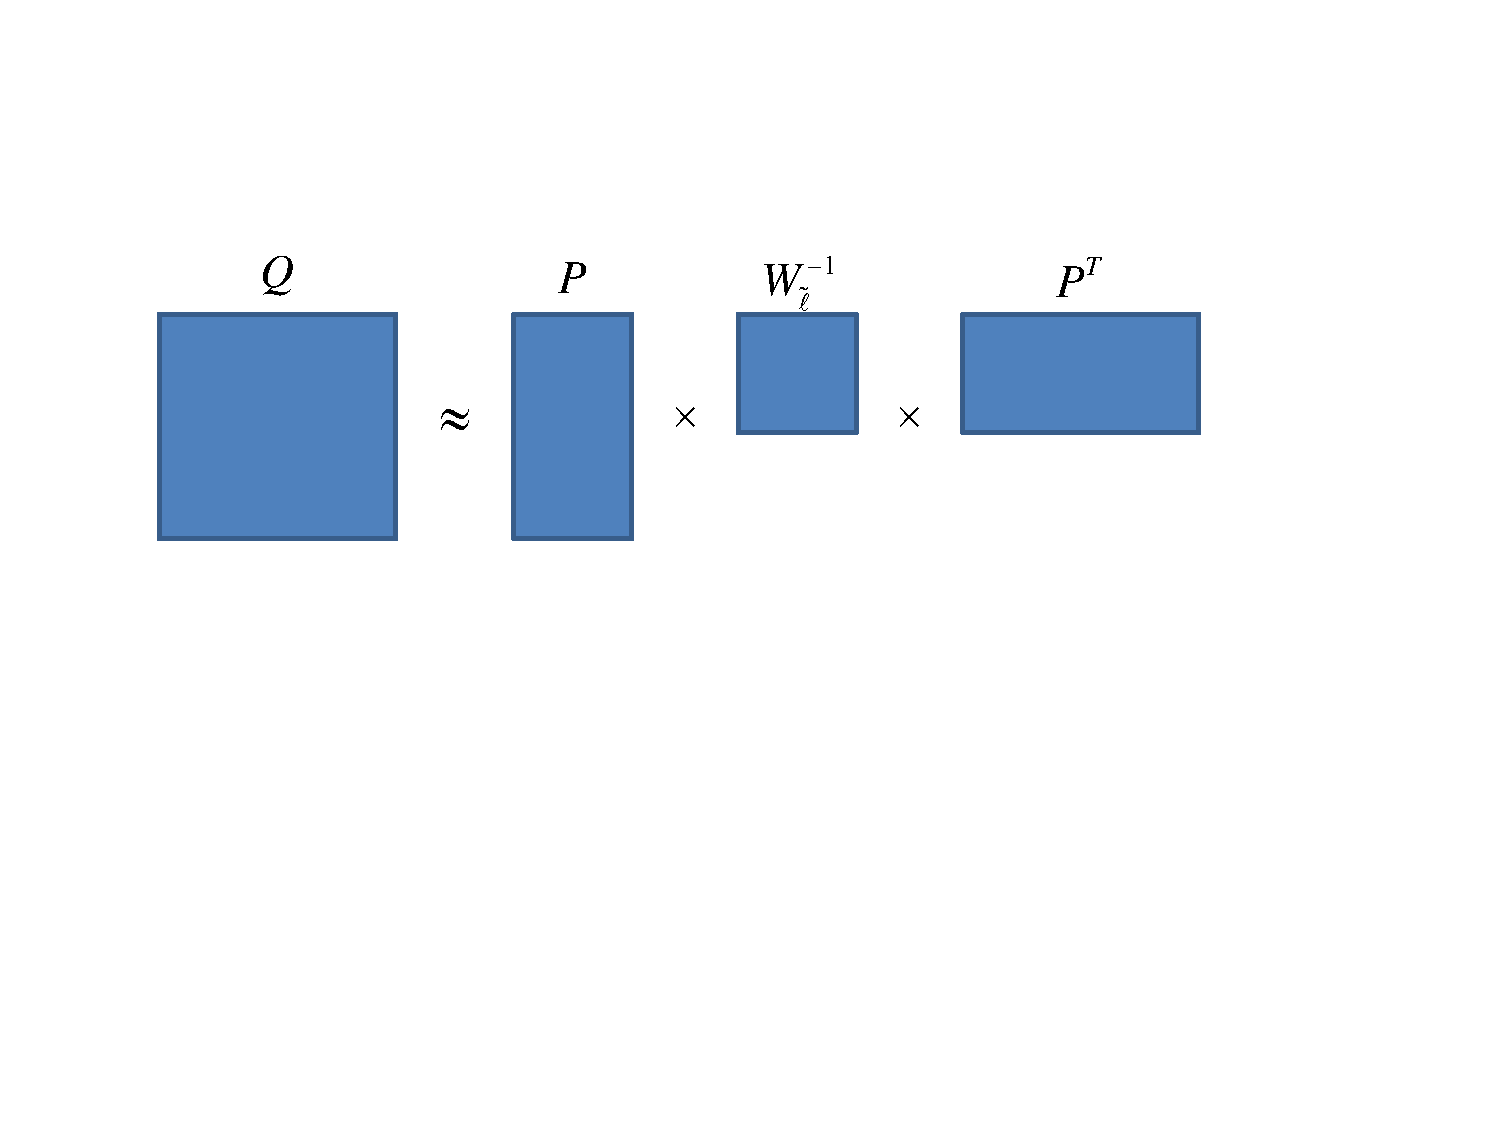
\includegraphics[width=3in]{nystrom.pdf}\\
\end{figure}


    \pause
    \item Time and space complexity:
    \item [] Time: Basis selection time + $O(\ell^2 \max(\tilde{\ell}, n))$ overall. (Alright...)
    \item [] Space: $O(\ell \max(\tilde{\ell}, n))$. (Good! But we don't know how large is $\tilde{\ell}$.)
    \pause
    \item Exists studies on how to get a compact and representative $B$.
  \end{itemize}
\end{frame}

\subsection{Nystr\"om Method for Linear Representation}
\begin{frame}
  \frametitle{An Equivalent Representation (1/2)}
  \begin{itemize}
    \item Bottleneck for the previous method: kernel matrix $Q$ of size $O(\ell^2)$. But observe the folliwing...
    \pause
    \item $Q = \tilde{X}^T\tilde{X}$ by Cholesky decomposition. (This is valid because $Q$ is PSD by definition.)
    \item Investigate the columns of $\tilde{X} = [\tilde{\bx}_1 \dots \tilde{\bx}_\ell]$. We have 
    $
    \tilde{\bx_i}^T \tilde{\bx_j} = 
    Q_{ij} = 
    \phi(\bx_i)^T \phi(\x_j) = K(\bx_i,\bx_j) 
    $.
    \pause
    \item We represent the kernelized linear products as regular linear products. Let's call $\tilde{X}$ a compact representation. 
  \end{itemize}
\end{frame}

\begin{frame}
  \frametitle{An Equivalent Representation (2/2)}
  \begin{itemize}
    \item Dual: 
    \begin{align}
    \min_{\balpha} \  &  \frac{1}{2} \balpha^T Q  \balpha - \be^T \balpha \nonumber \\
    \mbox{s.t.} \  & 0 \le \alpha_i \le C \quad \forall i \mbox{.} \nonumber
    \end{align}
    \pause
    \item Primal:
    \begin{equation}
      \min_{\bw, b}
      \frac{1}{2} \bw^T\bw + C\sum_{i=1}^\ell \max(1-y_i\bw^T\tilde{\bx}_i, 0) \nonumber
    \end{equation} 
    \pause
    \item Issue: computing $\tilde{\bx}_i$ requires the computation of the $\ell^2$-sized kernel.
  \end{itemize}
\end{frame}

\begin{frame}
  \frametitle{Nystr\"oms' Equivalent Representation}
  \begin{itemize}
    \item Let's go back to kernel approximation!
    \pause
    \item As $\tilde{Q} = P^TW^{-1}P$, we can find a matrix $R$ such that $W^{-1} = R^TR$, and $RP$ is our a compact representation.
    \pause
    \item [] Time: Basis selection time + $O(\ell \tilde{\ell} n)$ overall.
    \item [] Space: $O(\ell \max(\tilde{\ell}, n))$.
    \pause
    \item If we set our basis size, $\tilde{\ell}$, as $n$. The space consumption is optimal, but the speed still depends on the basis selection part.
  \end{itemize}
\end{frame}

\begin{frame}
  \frametitle{Another View of Basis Selection (1/2)}
  \begin{itemize}
    \item We view $RP$ as input data and do feature selection on it to get a more compact feature set.
    \item Recall that: $P_{:i} = [K(\bx_i, \bb_1), \dots, K(\bx_i, \bb_{\tilde{\ell}})]^T$
    \item This is not a basis selection algorithm because $R$ introduces dependency between dimensions.
    \pause
    \item We remove $R$! Each dimension is then independent of other basis vector, we can view $P$ as our linear SVM input data and do feature selection for basis selection. 
    \item L1-regularized linear SVM which runs linear time in data size is used in the work.
  \end{itemize}
\end{frame}

\begin{frame}
  \frametitle{Another View of Basis Selection (2/2)}
  \begin{itemize}
    \item Does it hurt by removing $R$?
    \pause
    \item Say $\bp_+$ and $\bp_-$ are two samples with different labels.
    \pause
    \item If for a $\bw$, $\bw^T\bp_+ > \bw^T\bp_-$ (separable), then
    $\bw^TR^{-1}R\bp_+  > \bw^TR^{-1}R\bp_-$.
    \pause
    \item $R^{-1}\bw$ separates $R\bp_+$ and $R\bp_-$.
    \pause
    \item When doing the linear tranformation by $R$, we preserve separability.
  \end{itemize}
\end{frame}

\begin{frame}
  \frametitle{A Linear Feature Selection Algorithm}
  \begin{itemize}
   \item []
    \begin{figure}
      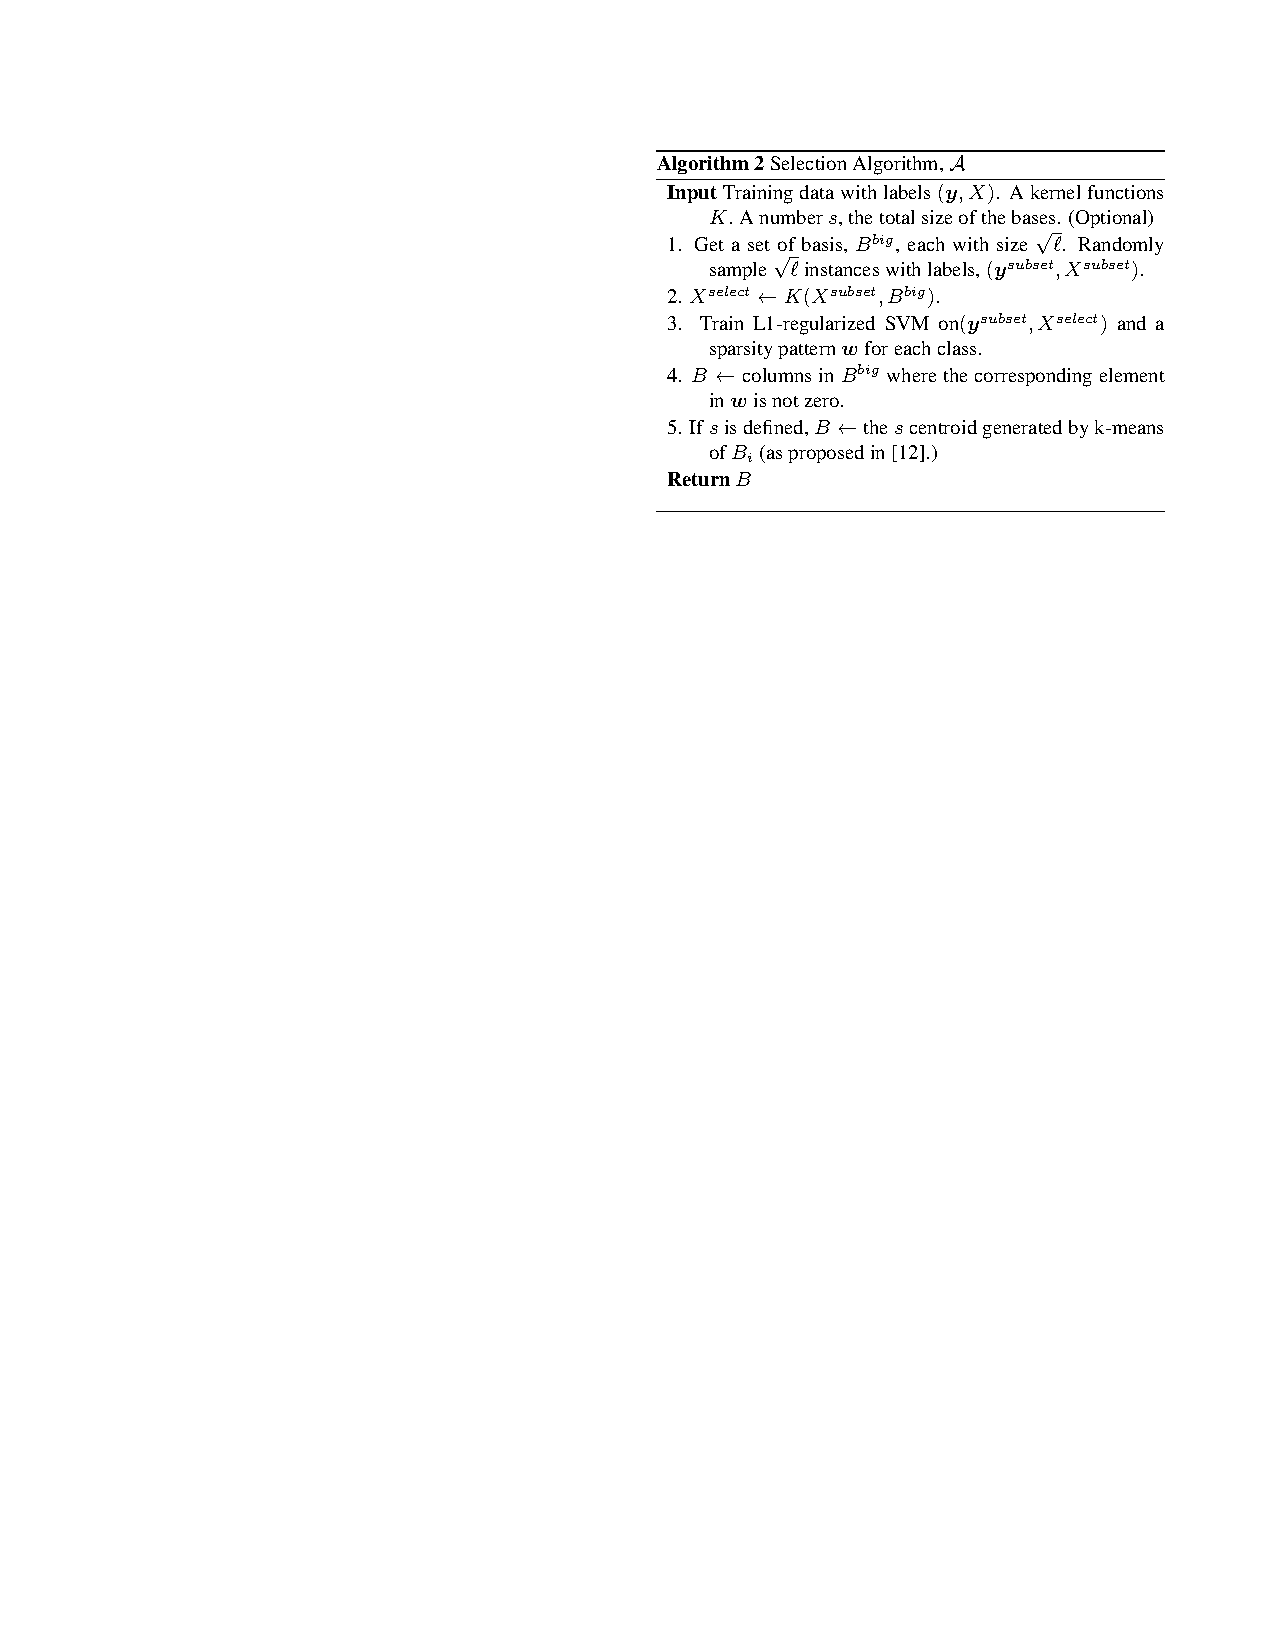
\includegraphics[width=3.2in]{algo2.pdf}\\
    \end{figure}
  \end{itemize}
\end{frame}

\begin{frame}
  \frametitle{The Algorithm Workflow}
  \begin{enumerate}
    \item Input data: $(\by, X)$, a kernel $K$.
    \item Run some basis selection algorithm in linear time and get the basis $B$.
    \item Compute the new data $\tilde{X} = K(X, B) \text{Chol}(K(B, B)^{-1})$.
    \item Train on $(\by, \tilde{X})$
    \pause
    \item [] Time: $O(\sqrt{\ell} \sqrt{\ell} n) + O(\ell \tilde{\ell} n)$ overall.
    \item [] Space: $O(\ell \max(\tilde{\ell}, n))$.
  \end{enumerate}
\end{frame}

%-----------------------------------------------
\subsection{Experiments and Conclusions}
%-----------------------------------------------
%-----------------------------------------------
\begin{frame}{Experimental Settings}
\begin{itemize}
  \item We conduct experiments on two benchmark datasets: USPS and MNIST.
  \item We randomly split 70\% of the data for training and the remaining 30\% for testing.
  \item Repeat random split five times.
  \item We perform a five-fold cross validation to select the parameters $\gamma$ and $C$.
\end{itemize}
\begin{table}
\caption{Dataset descriptions (with the number $\ell$ of instances and the dimension $d$ of the data). The sizes for storing the data $\ell d$ and the associated kernel matrices $\ell^2$ are also listed.}
\center{
%\scriptsize
%\small
\begin{tabular}{|l|l|l|l|l|}
\hline
      & $\ell$ & $d$ & kernel size $\ell^2$ & data size $\ell d$ \\
\hline
USPS & 7291 & 256 &   53M  & 2M \\
MNIST   & 60000  & 780  & 3.6G & 47M  \\
\hline
\end{tabular}
}
\label{tab:datasets}
\end{table}
\end{frame}



%-----------------------------------------------
\begin{frame}{Discussions}
\begin{itemize}
  \item Our method achieved improved accuracy than linear SVMs
  \item The time for training and testing using our proposed model is comparable to that of linear SVMs
  \item The standard nonlinear SVM utilizes the full kernel matrix whose time complexity is quadratically scaled-up with $\ell$.
\end{itemize}

\begin{table}
{\small
\caption{Comparisons of accuracy and computation time (in sec.) on three datasets. We denote our proposed Nystr\"om approximated SVM as Nystr\"om primal SVM below.}
\center{
  \scriptsize

\begin{tabular}{|l|l|l|l|}
\hline
USPS  & Accuracy & Training Time & Testing Time   \\
\hline
Nystr\"om primal SVM & $97.057 \pm 0.402$ & $3.764 $ & $0.320 $   \\
nonlinear SVM & $98.007 \pm 0.198$ & $14.507 $ & $4.129 $   \\
linear SVM & $95.009 \pm 0.275$ & $2.274 $ & $0.079 $   \\
\hline
MNIST  & Accuracy & Training Time & Testing Time   \\
\hline
Nystr\"om primal SVM & $93.833 \pm 0.115$ & $24.6092 $ & $2.006 $   \\
nonlinear SVM & $98.547 \pm 0.066$ & $3650.334 $ & $524.487 $   \\
linear SVM & $91.917 \pm 0.077$ & $14.510 $ & $0.381 $   \\
\hline
\end{tabular}
}
\label{tab:mrkl_with_others}
}\end{table}
\end{frame}

%-----------------------------------------------
\begin{frame}{Comparisons to Random Basis Selection}
\begin{itemize}
  \item To verify the effectiveness of our proposed basis selection approach, we compare the performance
\begin{itemize}
  \item Using the basis matrix determined by our method
  \item Using the random sampling strategy
\end{itemize}
\item We plot the recognition rates using these two different methods on the two datasets.
\item Our selection method yields higher accuracy than random sampling when choosing the same basis size for most scenarios.
\end{itemize}

\end{frame}
%-----------------------------------------------
\begin{frame}{Comparisons to Random Basis Selection}
\begin{figure}[h!]
\centering
\caption{Performance using our basis selection method (in blue) vs. random sampling (in green) on USPS (top) and MNIST (bottom) datasets.}
  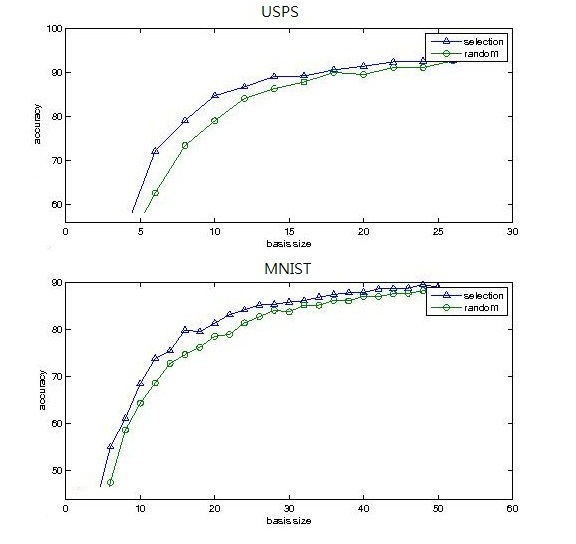
\includegraphics[width=6cm]{compare.jpg}
\label{fig:select}
\end{figure}
\end{frame}

%-----------------------------------------------
\begin{frame}{Conclusion}
\begin{itemize}
  \item We proposed a method to solve an approximated dual SVM in the primal based on Nystr\"om approximation.
  \item Our proposed method automatically determines the optimal basis matrix.
  \item The proposed method allows us to solve linear SVMs whose time complexity is simply scaling up with the dataset size.
  \item Experiments compared by linear SVM, our method
  \begin{itemize}
    \item achieved improved recognition accuracy
    \item reported comparable computation time
  \end{itemize}
  \item Both training and testing time using our approximated model was remarkably reduced compared to that of nonlinear SVMs.
\end{itemize}
\end{frame}
\end{document} 
